\documentclass[tikz]{standalone}
% \usetikzlibrary{intersections}
\usetikzlibrary{angles}
\input{./standalonepreamble.tex}

\begin{document}
\tikzset{help lines/.style=very thin}
\tikzset{Karl's grid/.style={help lines,color=blue!50}}

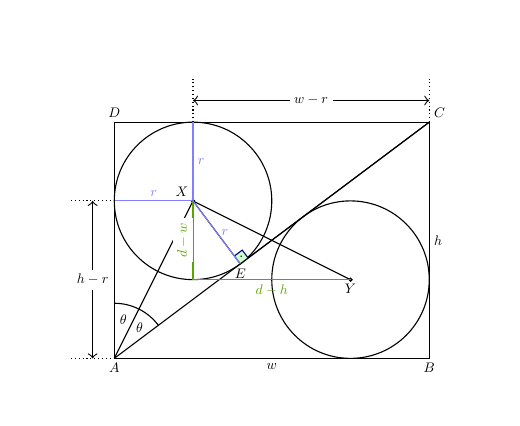
\begin{tikzpicture}[every node/.style={scale=0.5}]
  \clip (-1.1,-0.5) rectangle (4.8,4.2);
  \draw[thin] (0,0) rectangle (4,3);
  \draw (0,0) -- (4,3);
  \draw (1.0, 2.0) circle [radius=1cm];
  \draw (3.0, 1.0) circle [radius=1cm];
  \draw (1.0, 2.0) -- (3.0, 1.0);
  \filldraw (1.0, 2.0) circle [radius=0.2mm];
  \filldraw (3.0, 1.0) circle [radius=0.2mm];
  \draw (1.0,2.0) node[above left] {$X$};
  \draw (3.0,1.0) node[below] {$Y$};
  \draw (2.0,0.0) node[below] {$w$};
  \draw (4.0,1.5) node[right] {$h$};

  \draw[color=blue!50] (1.0,2) -- node[right] {$r$} (1.0,3);
  \draw[color=blue!50] (1.0,2) -- node[above] {$r$} (0.0,2);


  \draw[densely dotted] (-0.55,{3-1.0}) -- (0,{3-1});

  \draw[densely dotted] (-0.55,{0}) -- (0,0);
  \draw[<->] (-0.275,{0}) -- node[fill=white]{$h-r$} (-0.275,2);

  \draw[densely dotted] (1.0,3) -- (1.0,3.55);
  \draw[densely dotted] (4.0,3) -- (4.0,3.55);
  \draw[<->] (1.0,3.275) -- node[fill=white]{$w-r$} (4.0,3.275);

  \draw (1,2) -- (0,0);
  \draw[color=green!65!red] (1.0,2.0) -- node[above, rotate=90,fill=white]{$d-w$}(1.0,1.0);
  \draw[color=green!65!red] (1.0,1.0) -- node[below]{$d-h$} (3.0,1.0);


  \coordinate (A) at (0,0);
  \coordinate (B) at (4,0);
  \coordinate (C) at (4,3);
  \coordinate (D) at (0,3);
  \coordinate (E) at (1.6,1.2);
  \coordinate (X) at (1.0,2.0);

  \draw (A) node[below] {$A$};
  \draw (B) node[below] {$B$};
  \draw (C) node[above right] {$C$};
  \draw (D) node[above] {$D$};
  \draw (E) node[below] {$E$};

  \draw (C) -- (E) -- (X) pic [draw=blue!50!black, fill=green!20, 
          scale=0.5, angle eccentricity=.5, pic text=.] {right angle = C--E--X};
  \draw[color=blue!50, xshift=1cm, yshift=2cm, rotate=-53.13010235415598] (0,0)
          -- node[right] {$r$} (1.0,0.0);

  \draw (5.6mm,4.2mm) arc [start angle=36.86989764584402, end
          angle=63.43494882292201, radius=7mm];
  \draw (3.1304951684997055mm,6.260990336999411mm) arc [start angle=63.43494882292201, end angle=90, radius=7mm];
  \draw (50.152423234383015:5mm) node {$\theta$};
%   \draw (76.71747441146101:5mm) node[font=\large] {$\theta$};
  \draw (76.71747441146101:5mm) node[] {$\theta$};

%   \draw (C) -- (A) -- (X) pic [draw=black, angle radius=12mm, "$\theta$"] {angle = C--A--X};
\end{tikzpicture}

\end{document}
